\documentclass{article}
\usepackage[utf8]{inputenc}
\usepackage[spanish,mexico]{babel}
\usepackage{listings}
\usepackage{graphicx}
\usepackage{amsmath}

\title{Sólido de Revolución}
\author{
    Mauricio Chávez Olea\\315266847
    \and
    Frida Fernanda Lopez Perez\\315110520
}
\date{19 de Abril del 2019}

\begin{document}

\maketitle

\section*{Contorno de la botella con Desmos}

\begin{figure}[h!]
  \centering
  \includegraphics[width=0.7\textwidth]{desmos_botella.png}
  \caption{Funciones con la imagen}
  \label{fig:desmos_bottle}
\end{figure}

\begin{figure}[h!]
    \centering
    \includegraphics[width=0.7\textwidth]{desmos_contorno.png}
    \caption{Contorno de la botella}
    \label{fig:desmos_contour}
\end{figure}

\pagebreak

\section*{Sólido de revolución en Mathematica}

\lstset{language=Mathematica}
Código fuente en Mathematica
\begin{lstlisting}[frame=single]
coke = Piecewise[
  {
    {Sqrt[5x-(1/2)],  0 <= x <= 0.433},
    {Cos[1/3x]+0.32, 0.433 <= x <= 2.282},
    {Log10[x+1/2]+0.6, 2.282 <= x <= 4.717},
    {(0.9)Cos[1/2x + 4] + 0.42, 4.717 <= x <= 7.283},
    {(1)/(4) (x-7.9)^(2)+0.52, 7.283 <= x <= 8.465},
    {(-1)/(5) (x-8.5)^(2)+0.6, 8.465 <= x <= 9.199},
    {Sqrt[-2x+18.65], 9.199 <= x <= 9.325}
  }
];

RevolutionPlot3D[
    coke, 
    {x, 0, 9.325},
    RevolutionAxis->"X"
]
\end{lstlisting}

\begin{figure}[h!]
  \centering
  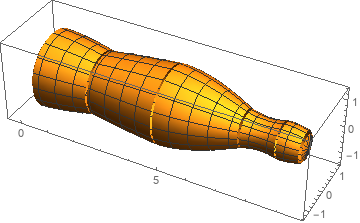
\includegraphics[width=1\textwidth]{coke_revolution.png}
  \caption{Funciones con la imagen}
  \label{fig:coke_revolution}
\end{figure}

\pagebreak

\section*{Calculando los volúmenes de cada función por el método del disco}

\begin{enumerate}
    \item $\sqrt{5 x-\frac{1}{2}}$
    $$ v = \pi \int_{0}^{0.433} (\sqrt{5 x-\frac{1}{2}})^2 dx$$
    
    Simplificando:
    $$ = \pi \int 5 x-\frac{1}{2} dx$$
    $$ = \pi (\int 5x dx - \int\frac{1}{2}dx) $$
    $$ = \pi (5\int x dx - \frac{1}{2}\int1 dx) $$
    $$ = 5\pi\int x dx - \frac{\pi}{2}\int1 dx $$
    
    Integrando:
    $$ = 5\pi\frac{x^2}{2} - \frac{\pi}{2}x $$
    
    Simplificando:
    $$ = \frac{5\pi x^2- \pi x}{2}$$
    $$ = \frac{\pi x (5x - 1)}{2}$$
    
    Sustituyendo intervalos:
    $$ = \frac{\pi (0.433) (5(0.433) - 1)}{2} - \frac{\pi 0 (5(0) - 1)}{2}$$
    $$ = \frac{\pi (0.433) (5(0.433) - 1)}{2} $$
    $$ = \frac{100889{\pi}}{400000} $$
    
    Por lo tanto, el resultado es:
    $$\frac{100889{\pi}}{400000} u^3 $$
    
    O aproximadamente $0.7923 u^3$
    
    \pagebreak
    \item $\cos \left(\frac{x}{3}\right)+0.32$
    $$ v = \pi \int_{0.433}^{2.282} (\cos \left(\frac{x}{3}\right)+0.32)^2 dx$$
    
    Simplificando:
    $$ = \pi \int \cos ^2\left(\frac{x}{3}\right)+0.64 \cos \left(\frac{x}{3}\right)+0.1024 dx $$
    $$ = \pi (\int \cos ^2\left(\frac{x}{3}\right) dx + \int 0.64 \cos \left(\frac{x}{3}\right) dx + \int 0.1024 dx) $$
    
    Integrando $\int \cos ^2\left(\frac{x}{3}\right) dx$:
    $$ = 3\int \cos^2(u)du$$
    $$ = 3(\frac{2-1}{2} \int \cos ^0 (u) du + \frac{\cos(u) \sin(u)}{2})$$
    
    Simplificando e integrando:
    $$ = 3(\frac{1}{2} \int 1 du + \frac{\cos(u) \sin(u)}{2})$$
    $$ = 3(\frac{u}{2} + \frac{\cos(u) \sin(u)}{2})$$
    $$ = \frac{3u}{2} + \frac{3 \cos(u) \sin(u)}{2}$$
    $$ = \frac{3u + 3\cos(u) \sin(u)}{2}$$
    Sustituyendo u:
    $$ = \frac{3(\frac{x}{3}) + 3\cos(\frac{x}{3}) \sin(\frac{x}{3})}{2}$$
    
    Simplificando:
    $$ = \frac{x}{2}+\frac{3}{4} \sin \left(\frac{2 x}{3}\right)$$
    
    Ahora integrando $\int 0.64 \cos \left(\frac{x}{3}\right) dx$:
    $$ = \frac{48}{25} \int \cos(u)du$$
    $$ = \frac{48}{25} \sin(u) $$
    
    Sustituyendo u:
    $$ = \frac{48}{25} \sin(\frac{x}{3}) $$
    
    Por último integrando $\int 0.1024 dx$:
    
    Simplificando:
    $$ = \int \frac{64}{625} dx$$
    
    Integrando:
    $$  = \frac{64}{625} x $$
    
    Sustituyendo las integrales resueltas:
    
    $$ = \pi(\frac{x}{2}+\frac{3}{4} \sin \left(\frac{2 x}{3}\right) + \frac{48}{25} \sin(\frac{x}{3}) + \frac{64}{625} x )$$
    
    Sustituyendo intervalos:
    $$ = \pi(\frac{2.282}{2}+\frac{3}{4} \sin \left(\frac{2 (2.282)}{3}\right) + \frac{48}{25} \sin(\frac{2.282}{3}) + \frac{64}{625} (2.282) ) $$
    $$- (\pi(\frac{0.433}{2}+\frac{3}{4} \sin \left(\frac{2 (0.433)}{3}\right) + \frac{48}{25} \sin(\frac{0.433}{3}) + \frac{64}{625} (0.433) ))$$
    
    Por lo tanto, el resultado es:
    $$ 8.4726 u^3 $$
    
    \pagebreak
    \item $\frac{\ln \left(x+\frac{1}{2}\right)}{\ln (10)}+0.6$
    $$ v = \pi \int_{4.717}^{2.282} (\frac{\ln \left(x+\frac{1}{2}\right)}{\ln (10)}+0.6)^2 dx$$
    
    \ Tomemos $u=x+\frac{1}{2}$ y $du=dx$, los limites cambian a $u=\frac{1}{2}+2.282=2.782$ y 
        $u=\frac{1}{2}+4.717=5.217$\vspace{.3cm}

        $\displaystyle\int_{2.782}^{5.217}(\frac{\log{u}}{log{10}}+\frac{3}{5})^2du = 
        \displaystyle\int_{2.782}^{5.217}(\frac{\log^2{u}}{\log^2{10}}+\frac{6\log{u}}{5\log{10}}
        +\frac{9}{25})du = ...$\vspace{.3cm}
        
        $... = \frac{6}{5\log{10}}\displaystyle\int_{2.782}^{5.217}(\log{u})du + 
        \frac{1}{\log^2{10}}\displaystyle\int_{2.782}^{5.217}(\log^2{u})du + 
        \frac{9}{25}\displaystyle\int_{2.782}^{5.217}(1)du = ...$\vspace{.3cm}

        $... = \left . \frac{6u\log{u}}{5\log{10}}\right |_{2.782}^{5.217} + 
        (\frac{9}{25} - \frac{6}{5\log{10}})\displaystyle\int_{2.782}^{5.217}(1)du + 
        \frac{1}{\log^2{10}}\displaystyle\int_{2.782}^{5.217}(\log^2{u})du = ...$\vspace{.3cm}

        $... = 3.0079 + \left . (u(\frac{9}{25} - \frac{6}{5\log{10}})) \right |_{2.782}^{5.217} + 
        \frac{1}{\log^2{10}}\displaystyle\int_{2.782}^{5.217}(\log^2{u})du = ...$\vspace{.3cm}

        $... = 2.61549 + \left . \frac{u\log^2{u}}{\log^2{10}} \right |_{2.782}^{5.217} - 
        \frac{2}{\log^2{10}}\displaystyle\int_{2.782}^{5.217}(\log{u})du = ...$\vspace{.3cm}

        $... = 4.75133 + \left . (-\frac{2u\log{u}}{\log^2{10}}) \right |_{2.782}^{5.217} + 
        \frac{2}{\log^2{10}}\displaystyle\int_{2.782}^{5.217}(1)du = ...$\vspace{.3cm}

        $... = 2.57414 + \left . \frac{2u}{\log^2{10}} \right |_{2.782}^{5.217} = 3.49268$
        
        
       \ Ahora multiplicamos el resultado por la constante:
       
       
        $3.49268\cdot \pi=10.972577829339999$
        
        Por lo tanto, el volumen es aproximadamente $10.9725 u^3$
    
    \pagebreak
    
    \item $0.9 \cos \left(\frac{x}{2}+4\right)+0.42$
    $$ v = \pi \int_{7.283}^{4.717} (0.9 \cos \left(\frac{x}{2}+4\right)+0.42)^2 dx$$
    
    Simplificando:
    $$ = \pi \int (\dfrac{9\cos\left(\frac{x}{2}+4\right)}{10}+\dfrac{21}{50})^2 dx$$
    $$ =  \frac{9}{2500} \pi \int (15 \cos(\frac{x}{2} + 4) + 7)^2$$
    
    Integrando $\int (15 \cos(\frac{x}{2} + 4) + 7)^2$:
    
    $$ =  2 \int (15 \cos(u) + 7)^2$$
    
    Resolviendo $\int (15 \cos(u) + 7)^2$:
    
    $$ = \int 225 \cos^2(u) + 210 \cos(u) + 49 dx$$
    $$ = 225 \int \cos^2(u) dx + 210 \int \cos(u) dx + 49 \int 1 dx$$
    
    Integrando $225 \int \cos^2(u) dx$:
    $$ = \frac{\cos(u) \sin(u)}{2} + \frac{1}{2} \int 1 du$$
    $$  =\frac{\cos(u) \sin(u)}{2} + \frac{1}{2} u$$
    
    Ahora integramos $ \int \cos(u) du $:
    $$ = \sin(u) $$
    
    Reemplazando las integrales resueltas de $\int (15 \cos(u) + 7)^2$:
    $$ = 225(\frac{\cos(u) \sin(u)}{2} + \frac{1}{2} u ) + 210\sin(u) + 49 u$$
    $$ = 225\frac{\cos(u) \sin(u)}{2} + \frac{225}{2} u + 210\sin(u) + 49 u$$
    $$ = 225\frac{\cos(u) \sin(u)}{2} + 210\sin(u) + \frac{323}{2} u$$
    
    Reemplazamos las integrales resueltas en $ 2 \int (15 \cos(u) + 7)^2 $
    $$ = 2(225\frac{\cos(u) \sin(u)}{2} + 210\sin(u) + \frac{323}{2} u )$$
    $$ = 225\cos(u) \sin(u)+ 420\sin(u) + 323 u )$$
    
    Deshaciendo la sustitución:
    $$ = 225\cos(\frac{x}{2} + 4) \sin(\frac{x}{2} + 4)+ 420\sin(\frac{x}{2} + 4) + 323 (\frac{x}{2} + 4) )$$
    
    Reemplazando la integral resuelta en $\frac{9}{2500} \pi \int (15 \cos(\frac{x}{2} + 4) + 7)^2$
    
    $$ = \frac{9}{2500} \pi (225\cos(\frac{x}{2} + 4) \sin(\frac{x}{2} + 4)+ 420\sin(\frac{x}{2} + 4) + 323 (\frac{x}{2} + 4) ))$$
    
    Sustituyendo los intervalos:
    
    $$ = \frac{9}{2500} \pi (225\cos(\frac{7.283}{2} + 4) \sin(\frac{7.283}{2} + 4)+ 420\sin(\frac{7.283}{2} + 4) + 323 (\frac{7.283}{2} + 4))$$
    $$ - (\frac{9}{2500} \pi (225\cos(\frac{4.717}{2} + 4) \sin(\frac{4.717}{2} + 4)+ 420\sin(\frac{4.717}{2} + 4) + 323 (\frac{4.717}{2} + 4)))$$
    
    Por lo tanto, el volumen es igual a:
    
    $$\frac{370287}{125000} \pi u^3$$
    
    O aproximadamente:
    
    $$9.3063 u^3$$
    
    \pagebreak
    
    
    \item $\frac{1}{4} (x-7.9)^2+0.52$
    $$ v = \pi \int_{4.717}^{7.283} (\frac{1}{4} (x-7.9)^2+0.52)^2 dx$$
    
    Expandiendo:
    $$ = \pi(\int \dfrac{x^4}{16}-\dfrac{79x^3}{40}+\dfrac{18923x^2}{800}-\dfrac{508839x}{4000}+\dfrac{41486481}{160000} dx) $$
    
    Simplificando:
    $$ = {\pi}( \dfrac{{1}}{16}\int x^4 dx -\dfrac{79}{40} \int x^3 dx + \dfrac{18923}{800} \int x^2 dx - \dfrac{508839}{4000} \int x dx  + \dfrac{41486481}{160000} \int 1 dx )  $$
    
    Resolviendo las integrales:
    $$ = {\pi}( \dfrac{{1}}{16}(\frac{x^5}{5}) -\dfrac{79}{40} (\frac{x^4}{4}) + \dfrac{18923}{800} (\frac{x^3}{3}) - \dfrac{508839}{4000} (\frac{x^2}{2})  + \dfrac{41486481}{160000} x )  $$
    
    $$ = \pi(\dfrac{x^5}{80}-\dfrac{79x^4}{160}+\dfrac{18923x^3}{2400}-\dfrac{508839x^2}{8000}+\dfrac{41486481}{160000}x)$$
    
    Sustituyendo los intervalos:
    $$ = \pi(\dfrac{(8.465)^5}{80}-\dfrac{79(8.465)^4}{160}+\dfrac{18923(8.465)^3}{2400}-\dfrac{508839(8.465)^2}{8000}+\dfrac{41486481}{160000}(8.465)) $$
    
    $$ -(\pi(\dfrac{(7.283)^5}{80}-\dfrac{79(7.283)^4}{160}+\dfrac{18923(7.283)^3}{2400}-\dfrac{508839(7.283)^2}{8000}+\dfrac{41486481}{160000}(7.283))) $$
    
    Por lo tanto, el resultado es:
    
    $$\dfrac{13277654599067991}{40000000000000000} \pi u^3 $$
    
    O aproximadamente:
    
    $$ 1.0428 u^3 $$
    
    
    \pagebreak

    
    \item $0.6 -\frac{1}{5} (x-8.5)^2$
    $$ v = \pi \int_{8.465}^{9.199} (0.6\, -\frac{1}{5} (x-8.5)^2)^2 dx $$
    
    Simplificando:
    $$ = \pi {\displaystyle\int}\left(\dfrac{3}{5}-\dfrac{\left(x-\frac{17}{2}\right)^2}{5}\right)^2\,\mathrm{d}x$$
    $$ = \frac{1}{400} \pi \int ((2x - 17)^2 - 12)^2 dx $$

    Sustituyendo por u:
    
    $$ = \frac{1}{400} \frac{1}{2} \pi \int (u^2 - 12)^2 du $$
    $$ = \frac{1}{800} \pi \int (u^2 - 12)^2 du $$
    
    Integrando $ \int (u^2 - 12)^2 du $
    
    Expandiendo:
    $$={\displaystyle\int}\left(u^4-24u^2+144\right)\mathrm{d}u$$
    
    Simplificando:
    $$ = \int u^4 du - 24 \int u^2 du + 144 \int 1 du $$
    
    Resolviendo las integrales:
    $$ = \frac{u^5}{5} - 24 (\frac{u^3}{3}) + 144u $$
    $$ = \frac{u^5}{5} - 8u^3 + 144u $$
    
    Reemplazando las integrales resueltas en $\frac{1}{800} \pi \int (u^2 - 12)^2 du $\\
    
    Deshaciendo la sustitución:
    $$ = \frac{1}{800} \pi (\frac{(2x-17)^5}{5} - 8(2x-17)^3 + 144(2x-17)) $$
    
    Simplificando:
    $$ = \frac{(2x-17)^5 \pi}{4000} - \frac{8\pi(2x-17)^3}{800} + \frac{144\pi(2x-17)}{800} $$
    
    Sustituyendo los intervalos:
    $$ = \frac{(2(9.199)-17)^5 \pi}{4000} - \frac{8\pi(2(9.199)-17)^3}{800} + \frac{144\pi(2(9.199)-17)}{800} $$
    $$ - (\frac{(2(8.465)-17)^5 \pi}{4000} - \frac{8\pi(2(8.465)-17)^3}{800} + \frac{144\pi(2(8.465)-17)}{800}) $$
    
    Por lo tanto, el resultado es:
    
    $$ \dfrac{14890561618812687{\pi}}{62500000000000000} u^3 $$
    
    O aproximadamente $0.7484 u^3$
    
    \pagebreak
    \item $\sqrt{18.65 -2 x}$
    $$ v = \pi \int_{9.199}^{9.325} (\sqrt{18.65 -2 x})^2 dx $$
    
    Simplificando:
    $$ = \pi \int 18.65 -2x dx $$
    $$ = \pi (18.65 \int 1 dx - 2 \int x dx) $$
    
    Resolviendo las integrales:
    $$ = \pi (18.65x - 2 \frac{x^2}{2} dx) $$
    
    Simplificando:
    $$ = \pi (18.65x - x^2) $$
    $$ = 18.65\pi x - \pi x^2 $$
    $$ = \pi x (18.65 - x)  $$
    
    Sustituyendo los intervalos:
    $$ = 9.325 \pi  (18.65 - 9.325) - (9.199 \pi (18.65 - 9.199))  $$
    
    Por lo tanto, el resultado es:
    $$ \frac{3969\pi}{250000} $$
    
    Lo que es aproximadamente: $0.0498 u^3$
    
    \section*{Volumen total de la botella}
    
    Para calcular el volumen total, solo basta con sumar los individuales:
    
    $$ 0.7923 + 8.4726 + 10.9725 + 9.3063 + 1.0428 + 0.7484 + 0.0498 $$
    
    Lo que nos da como resultado $31.3847$, por lo que el volumen total de la botella es $31.3847 u^3$
    
\end{enumerate}

\end{document}
